%%%%%%%%%%%%%%%%%%%%%%%%%%%%%%%%%%%%%%%%%%%%%%%%%%%%%%%%
%   |------------------------------------------|       %
%   |Aplicación de comercio electrónico para   |       %
%   |teléfonos móviles con S.O. Android        |       %
%   |                                          |       %
%   | Proyecto de graduación                   |       %
%   |__________________________________________|       %
%                                                      %
%   Autores                                            %
%   -------                                            %
%                                                      %
% * Soto, Paula Fabiana (CX05-0967-4)                  %
%     paulette255@gmail.com                            %
% * Vallejo, Sergio Daniel (CX05-0392-4)               %
%     vallejosergio@gmail.com                          %
%                                                      %
%   Tutor                                              %
%   -------                                            %
%                                                      %
% * Ing. Augusto Maximiliano Odstrcil                  %
%        modstrcil@gmail.com                           %
%                                                      %
%                                                      %
%%%%%%%%%%%%%%%%%%%%%%%%%%%%%%%%%%%%%%%%%%%%%%%%%%%%%%%%

\chapter{Disciplina de Implementación}
\label{chap:implementacion}

\section{Arquitectura de la aplicación}

\begin{figure}[H]
  \centering
    %lo que agregué entre corchetes hace que el ancho de la imagen ocupe el 80% del área de texto. Si sacás eso la imagen no se redimensiona y se va de la hoja. Se puede usar algo parecido para limitar el alto si es necesario.
    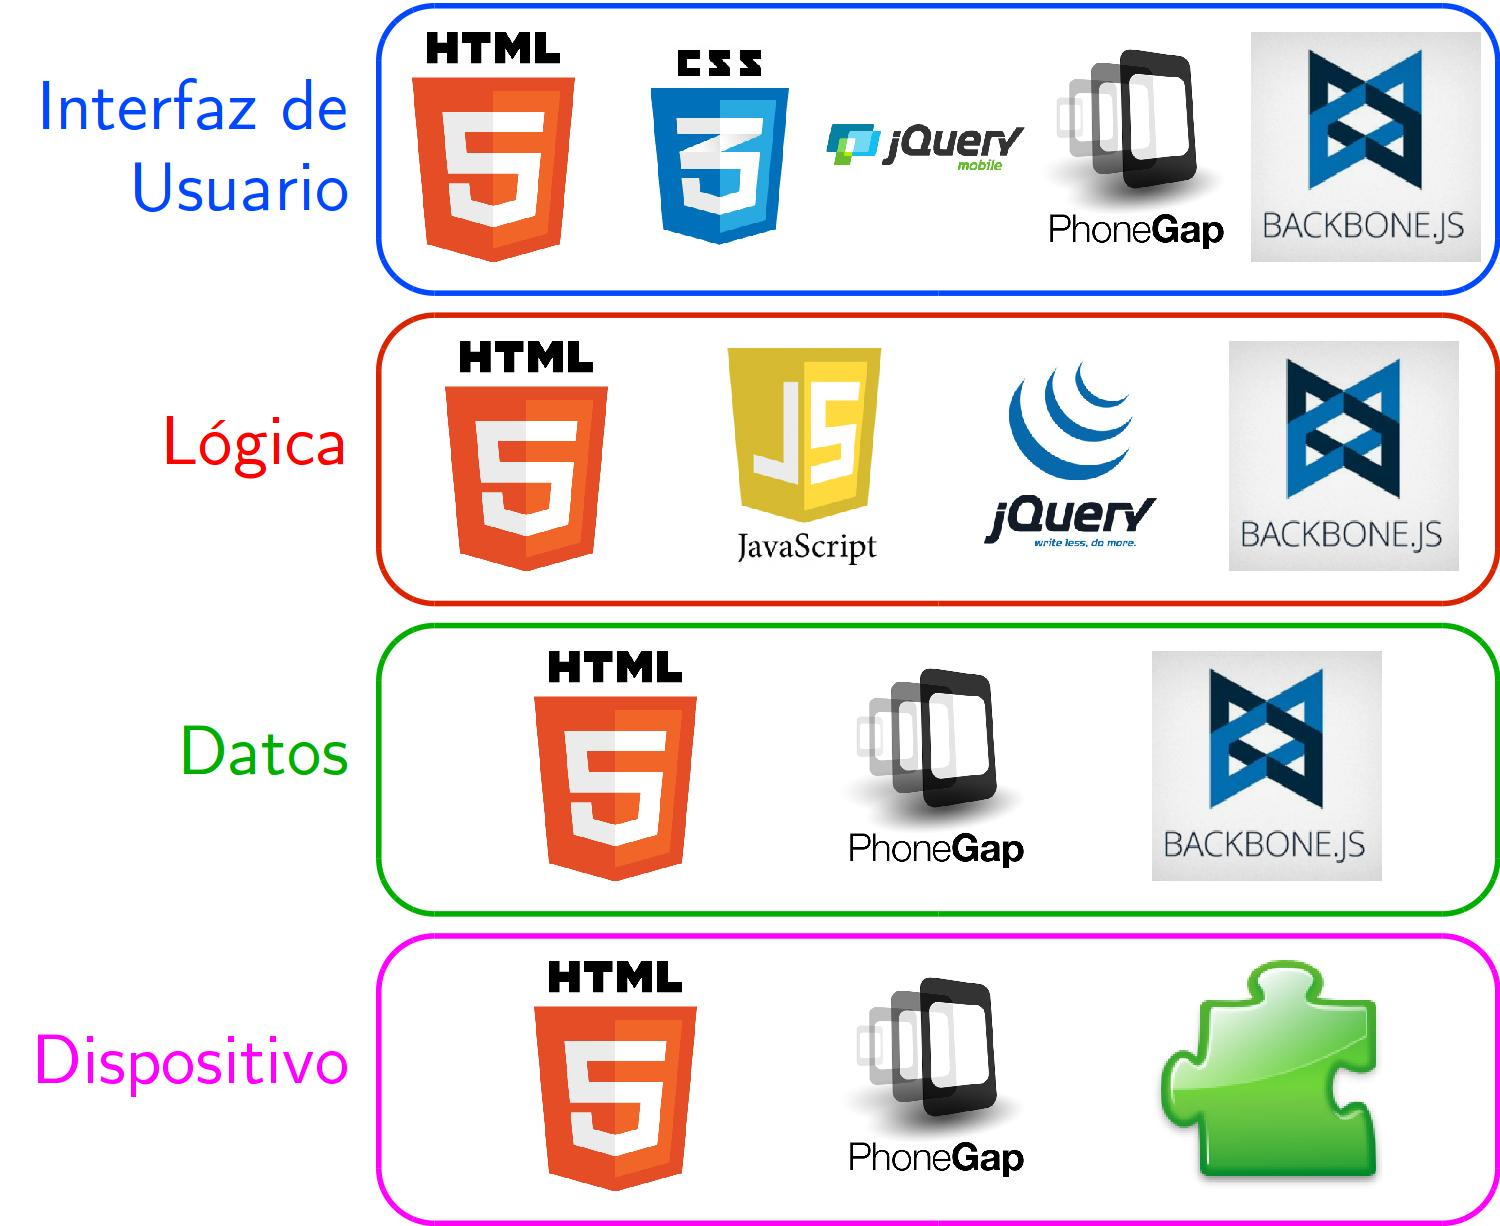
\includegraphics[width=1\textwidth]{imagenes/implementacion/arquitectura.jpg}
    
     \caption{Arquitectura de la aplicación, mostrando los frameworks utilizados}
    \label{fig:arquitectura-aplicacion}
\end{figure}

\section{Diagrama de Despliegue}

 \begin{figure}[H]
  \centering
    %lo que agregué entre corchetes hace que el ancho de la imagen ocupe el 80% del área de texto. Si sacás eso la imagen no se redimensiona y se va de la hoja. Se puede usar algo parecido para limitar el alto si es necesario.
    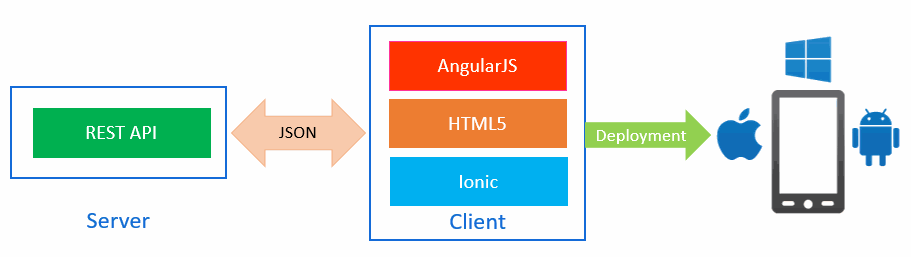
\includegraphics[width=1\textwidth]{imagenes/implementacion/despliegue.png}
    \label{diagrama-despliegue}
\end{figure}

\section{Elección del Lenguaje}

    Independientemente del paradigma de ingeniería de software, el lenguaje de programación tendrá impacto en la planificación, el análisis, el diseño, la codificación, la prueba y el mantenimiento de un proyecto. Para la construcción de la aplicación se eligió la utilización de los lenguajes web HTML5, CSS3 y JavaScript.

    La elección de estos lenguajes para la construcción de la apliación se debe a las siguientes ventajas que ofrecen:
    \begin{itemize}
        \item \emph{Mayor portabilidad:} Al ser tecnologías estándares y soportadas por la mayoría de los teléfonos celulares modernos, es posible que una misma aplicación sea muy fácilmente adaptable a varias plataformas móviles.
        \item \emph{Soporte futuro:} Todas las plataformas móviles están trabajando para mejorar el soporte que ofrecen a las tecnologías web, ofreciendo una mejor experiencia al usuario.
        \item \emph{Aprovechamiento de conocimiento de desarrollo de aplicaciones web:} Desarrollando aplicaciones móviles en \gls{HTML}5, \gls{CSS}3 y \gls{JavaScript} es posible aplicar el conocimiento en el desarrollo de aplicaciones web desarrolladas para navegadores en equipos de escritorio 
    \end{itemize}
   
\section{Arquitectura de Android}

Los componentes principales del sistema operativo Android, que pueden verse en la figura \ref{fig:arquitectura-android}, son:

\begin{itemize}
    \item \emph{Aplicaciones:} las aplicaciones base incluyen un cliente de correo electrónico, programa de SMS, calendario, mapas, navegador, contactos y otros. La mayoría de las aplicaciones están escritas en lenguaje de programación \gls{Java}, aunque existen \gls{framework}s para desarrollar aplicaciones en otros lenguajes como \gls{HTML}, \gls{CSS} y \gls{JavaScript} o \gls{Python}.
    \item \emph{Marco de trabajo de aplicaciones:} los desarrolladores tienen acceso completo a los mismos APIs del framework usados por las aplicaciones base. La arquitectura está diseñada para simplificar la reutilización de componentes; cualquier aplicación puede publicar sus capacidades y cualquier otra aplicación puede luego hacer uso de esas capacidades (sujeto a reglas de seguridad del framework). Este mismo mecanismo permite que los componentes sean reemplazados por el usuario.
    \item \emph{Bibliotecas:} Android incluye un conjunto de bibliotecas de C/C++ usadas por varios componentes del sistema. Estas características se exponen a los desarrolladores a través del marco de trabajo de aplicaciones de Android; algunas son: System C library (implementación biblioteca C estándar), bibliotecas de medios, bibliotecas de gráficos, 3D y SQLite, entre otras.
    \item \emph{Runtime de Android:} Android incluye un set de bibliotecas base que proporcionan la mayor parte de las funciones disponibles en las bibliotecas base del lenguaje Java. Cada aplicación Android corre su propio proceso, con su propia instancia de la máquina virtual Dalvik. Dalvik ha sido escrito de forma que un dispositivo puede correr múltiples máquinas virtuales de forma eficiente. Dalvik ejecuta archivos en el formato Dalvik Executable (.dex), el cual está optimizado para minimizar el consumo de memoria. La Máquina Virtual está basada en registros y corre clases compiladas por el compilador de Java que han sido transformadas al formato.dex por la herramienta incluida "dx".
    
    \item \emph{Núcleo \gls{Linux}:} Android depende de Linux para los servicios base del sistema como seguridad, gestión de memoria, gestión de procesos, pila de red y modelo de controladores. El núcleo también actúa como una capa de abstracción entre el hardware y el resto de la pila de software.
   
 \end{itemize}

\begin{figure}[htbp]
  \centering
    %lo que agregué entre corchetes hace que el ancho de la imagen ocupe el 80% del área de texto. Si sacás eso la imagen no se redimensiona y se va de la hoja. Se puede usar algo parecido para limitar el alto si es necesario.
    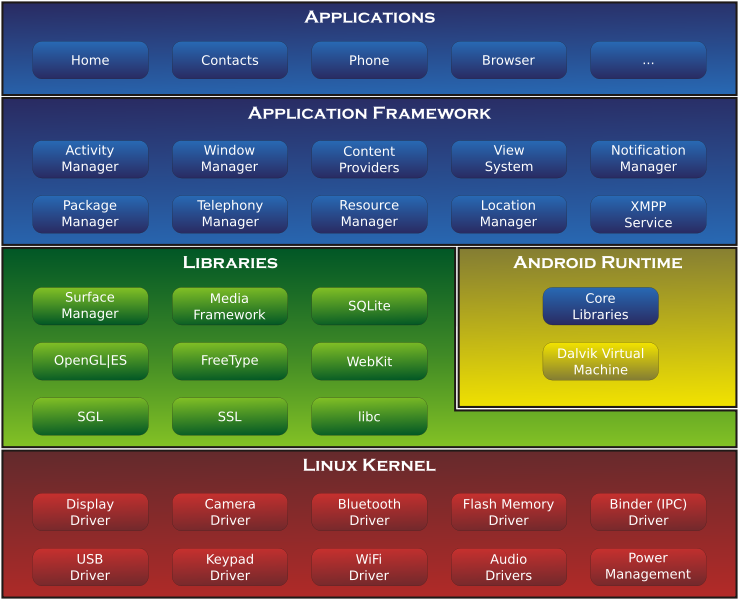
\includegraphics[width=0.8\textwidth]{imagenes/arquitecturaAndroid.png}
    
     \caption{Arquitectura de Android}
    \label{fig:arquitectura-android}
\end{figure}

\section{PhoneGap}

\begin{figure}[htbp]
  \centering
    %lo que agregué entre corchetes hace que el ancho de la imagen ocupe el 80% del área de texto. Si sacás eso la imagen no se redimensiona y se va de la hoja. Se puede usar algo parecido para limitar el alto si es necesario.
    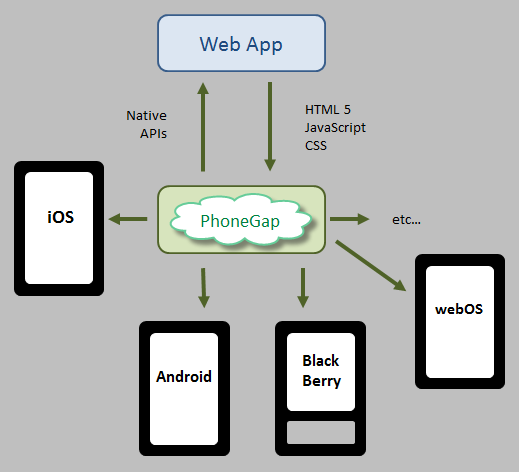
\includegraphics[width=0.5\textwidth]{imagenes/phonegap.png}
    
     \caption{Arquitectura de PhoneGap}
    \label{arquitectura-phonegap}
\end{figure}

PhoneGap es un \gls{framework} de código abierto que actúa como un intermediario entre las aplicaciones web y los dispositivos móviles. Permite crear aplicaciones móviles instalables utilizando tecnología web: \gls{JavaScript}, \gls{HTML}5 y \gls{CSS}3.

Las aplicaciones resultantes no son totalmente nativas, ni puramente basado en la web. La desventaja de que una aplicación sea totalmente nativa es que sólo se podrá utilizar para la plataforma para la que fue realizada, es decir si se hace una aplicación para Android luego no se podrá reutilizar el código para hacer la misma aplicación para iOS.

Con PhoneGap se puede reutilizar el código de una aplicación para crear el paquete instalable de cualquiera de las 7 plataformas móviles soportadas: iOS, Android, Blackberry, Windows Phone, WebOS de Palm, Symbian y Bada.

PhoneGap permite acceder a funciones nativas como el acelerómetro, cámara, brújula, contactos, archivos, ubicación geográfica, almacenamiento  y notificaciones.

PhoneGap para Android esta dividido en dos partes:

\begin{itemize}
    \item \emph{Librerías nativas (phonegap.jar):} Agrega acceso JavaScript para APIs nativas.
    
    \item \emph{Archivos javascript (phonegap.js):} Contenedores JavaScript para llamados de APIs nativas.
    
   
 \end{itemize}
\subsection{Ventajas de PhoneGap}

\begin{itemize}

    \item Soporta 7 plataformas móviles: iOS, Android, Blackberry, Windows Phone, WebOS de Palm, Symbian y Bada.
    
    \item Acceso a características nativas de cada plataforma a través de su API, a las que una aplicación web visitada desde el navegador no podría acceder, como acceso a la cámara de fotos, acelerómetro, notificaciones, etc.
    
    \item Permite ejecutar a través de JavaScript plugins escritos en código nativo.
    
    \item Permite distribuir aplicaciones realizadas utilizando HTML5 y JavaScript a través de las tiendas de aplicaciones oficiales de cada plataforma.
    
    \end{itemize}
    \subsection{Desventaja de phoneGap}
    \begin{itemize}
\item Normalmente las aplicaciones realizadas con PhoneGap tienen un menor rendimiento en tareas que requieren alta capacidad de procesamiento, sobre todo en versiones antiguas de las plataformas sobre las que se usa.

\item Se pierde la posibilidad de acceder a algunas características nativas, como los diferentes elementos de interfaz de usuario propios de cada plataforma, aunque estos pueden imitarse mediante el uso de CSS.
\end{itemize}

\section{Web services}
\label{sec:webservices}

Un servicio web (en inglés, Web service) es una tecnología que utiliza un conjunto de protocolos y estándares que sirven para intercambiar datos entre aplicaciones. Distintas aplicaciones de software desarrolladas en lenguajes de programación diferentes, y ejecutadas sobre cualquier plataforma, pueden utilizar los servicios web para intercambiar datos en redes de ordenadores como Internet. La interoperabilidad se consigue mediante la adopción de estándares abiertos.

Las ventajas de los servicios web son:

\begin{itemize}
    \item Aportan interoperabilidad entre aplicaciones de software independientemente de sus propiedades o de las plataformas sobre las que se instalen.
    \item Los servicios Web fomentan los estándares y protocolos basados en texto, que hacen más fácil acceder a su contenido y entender su funcionamiento.
    \item Permiten que servicios y software de diferentes compañías ubicadas en diferentes lugares geográficos puedan ser combinados fácilmente para proveer servicios integrados.
   
 \end{itemize}
 
\subsection{Razones para crear servicios Web}

La principal razón para usar servicios Web es que se pueden utilizar con HTTP sobre \gls{TCP} en el puerto 80. Dado que las organizaciones protegen sus redes mediante firewalls -que filtran y bloquean gran parte del tráfico de Internet, cierran casi todos los puertos TCP salvo el 80, que es, precisamente, el que usan los navegadores. Los servicios Web utilizan este puerto, por la simple razón de que no resultan bloqueados. Es importante señalar que los servicios web se pueden utilizar sobre cualquier protocolo, sin embargo, TCP es el más común.

Otra razón por la que los servicios Web son muy prácticos es que pueden aportar gran independencia entre la aplicación que usa el servicio Web y el propio servicio. De esta forma, los cambios a lo largo del tiempo en uno no deben afectar al otro. Esta flexibilidad será cada vez más importante, dado que la tendencia a construir grandes aplicaciones a partir de componentes distribuidos más pequeños es cada día más utilizada.
Se pueden desarrollar servicios web como parte de una aplicación web, permitiendo acceder a los mismos datos que esta.


\subsection{REST}



REST es una técnica de arquitectura software para sistemas hipermedia distribuidos como la World Wide Web.
REST describe cualquier interfaz web simple que utiliza \gls{XML} (o \gls{JSON}) y HTTP, sin las abstracciones adicionales de los protocolos basados en patrones de intercambio de mensajes como el protocolo de servicios web \gls{SOAP}. 

Los sistemas que siguen los principios REST se llaman con frecuencia RESTful.

\begin{figure}[htbp]
  \centering
    %lo que agregué entre corchetes hace que el ancho de la imagen ocupe el 80% del área de texto. Si sacás eso la imagen no se redimensiona y se va de la hoja. Se puede usar algo parecido para limitar el alto si es necesario.
    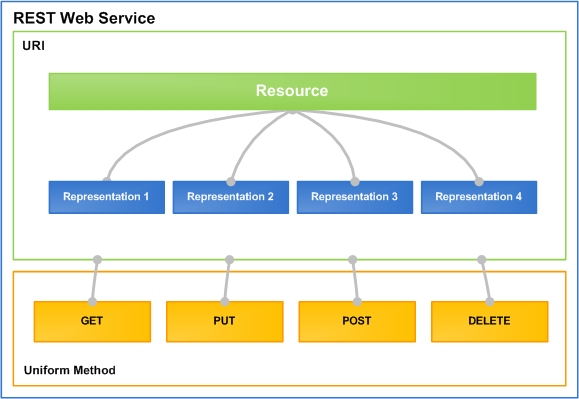
\includegraphics[width=0.8\textwidth]{imagenes/REST.jpg}
    
     \caption{Web Services REST}
    \label{fig:REST}
\end{figure}

REST afirma que la web ha disfrutado de escalabilidad como resultado de una serie de diseños fundamentales clave:

\begin{itemize}
    \item \emph{Un protocolo cliente/servidor sin estado:} cada mensaje HTTP contiene toda la información necesaria para comprender la petición. Como resultado, ni el cliente ni el servidor necesitan recordar ningún estado de las comunicaciones entre mensajes. Sin embargo, en la práctica, muchas aplicaciones basadas en HTTP utilizan cookies y otros mecanismos para mantener el estado de la sesión (algunas de estas prácticas, como la reescritura de URLs, no son permitidas por REST)
    
    \item \emph{Un conjunto de operaciones bien definidas que se aplican a todos los recursos de información:} HTTP en sí define un conjunto pequeño de operaciones, las más importantes son POST, GET, PUT y DELETE.
    
    \item Una sintaxis universal para identificar los recursos. En un sistema REST, cada recurso es direccionable únicamente a través de su \gls{URI}.
    \item El uso de hipermedios, tanto para la información de la aplicación como para las transiciones de estado de la aplicación: la representación de este estado en un sistema REST son típicamente \gls{HTML}, XML o JSON. Como resultado de esto, es posible navegar de un recurso REST a muchos otros, simplemente siguiendo enlaces sin requerir el uso de registros u otra infraestructura adicional.
   
 \end{itemize}
 
 \subsubsection{Recursos}
 Un concepto importante en REST es la existencia de recursos (elementos de información), que pueden ser accedidos utilizando un identificador global (un Identificador Uniforme de Recurso).
 
 Para manipular estos recursos, los componentes de la red (clientes y servidores) se comunican a través de una interfaz estándar (HTTP) e intercambian representaciones de estos recursos (los ficheros que se descargan y se envían.
 
La petición puede ser transmitida por cualquier número de conectores (por ejemplo clientes, servidores, cachés, túneles, etc.) pero cada uno lo hace sin "ver más allá" de su propia petición. Así, una aplicación puede interactuar con un recurso conociendo el identificador del recurso y la acción requerida, no necesitando conocer si existen cachés, proxys, cortafuegos, túneles o cualquier otra cosa entre ella y el servidor que guarda la información. La aplicación, sin embargo, debe comprender el formato de la información devuelta (la representación), que es por lo general un documento \gls{HTML}, \gls{XML} o \gls{JSON}, aunque también puede ser una imagen o cualquier otro contenido.


\section{Características de seguridad}

\subsection{Canal de comunicación cifrado}

En todos los casos en los que se realiza transferencia de datos confidenciales del usuario, como sus credenciales de acceso, datos personales u operaciones realizadas, es necesario asegurar que tanto las solicitudes y las respuestas se envían a través de un canal de comunicación cifrado.

La utilización de protocolos de comunicación inseguros, como HTTP, pueden hacer que la comunicación pueda ser interceptada utilizando ataques \gls{Man-in-the-middle}, permitiendo que el atacante pueda ver todos los datos intercambiados e incluso manipularlos o generar solicitudes falsas.

Para mitigar este riesgo, las comunicaciones de la aplicación se realizan utilizando el protocolo de comunicación segura \gls{HTTPS}. Este está basado en HTTP, pero  utiliza un cifrado basado en \gls{SSL/TLS} para crear un canal cifrado (cuyo nivel de cifrado depende del servidor remoto) más apropiado para el tráfico de información sensible que el protocolo HTTP. De este modo se consigue que la información sensible no pueda ser usada por un atacante que haya conseguido interceptar la transferencia de datos de la conexión, ya que lo único que obtendrá será un flujo de datos cifrados que le resultará imposible de descifrar, como se muestra en la figura \ref{fig:https}.

\begin{figure}[htbp]
  \centering
    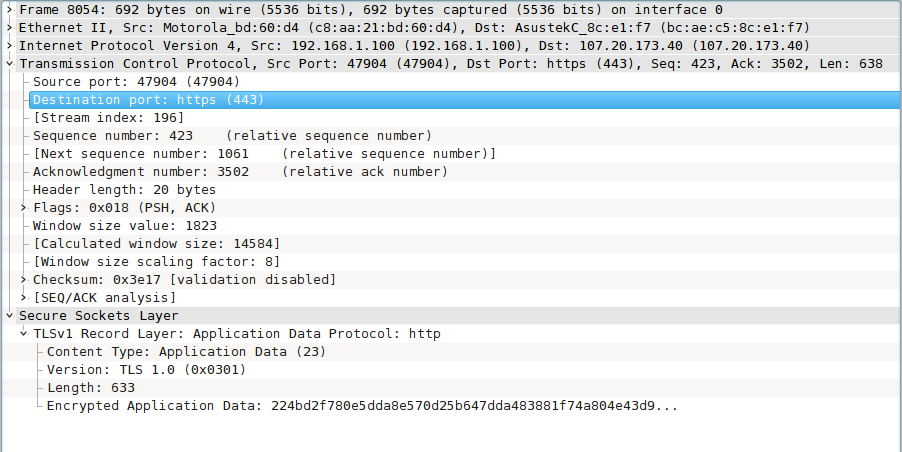
\includegraphics[width=0.9\textwidth]{imagenes/implementacion/https.png}
     \caption{Captura de la solicitud cifrada como lo vería un atacante utilizando Wireshark}
    \label{fig:https}
\end{figure}

\subsection{ACL para cada objeto}

Como ya se habló anteriormente, los Web services pueden ser públicamente accedidos a través de Internet, por lo que es imprescindible contar con un mecanismo que impida la realización de consultas o modificaciones no autorizadas. En la aplicación es necesario que los datos estén definidos correctamente: sólo un vendedor puede realizar la modificación de los datos de una tienda y de sus productos, sólo puede modificar los datos personales el usuario al que pertenece la cuenta activa y las órdenes no pueden modificarse una vez creadas y sólo pueden ser vistas por el usuario comprador o el vendedor.

Para asegurar que los datos sólo son accesibles por usuarios que están autorizados a leerlos o modificarlos se implementó un \gls{ACL} para cada objeto. Este dato se almacena cuando el objeto es creado, y está representado con un listado en formato \gls{JSON} incluyendo los permisos de los usuarios sobre ese objeto. En el siguiente ejemplo se muestra el caso de un objeto que es visible públicamente pero sólo el usuario con id \texttt{idUsuario} puede realizar modificaciones:

\begin{verbatim}
{
    "idUsuario":
        {
            "read":true,
            "write":true
        },
    "*":
        {
            "read":true
        }
}
\end{verbatim}

\begin{figure}[htbp]
  \centering
    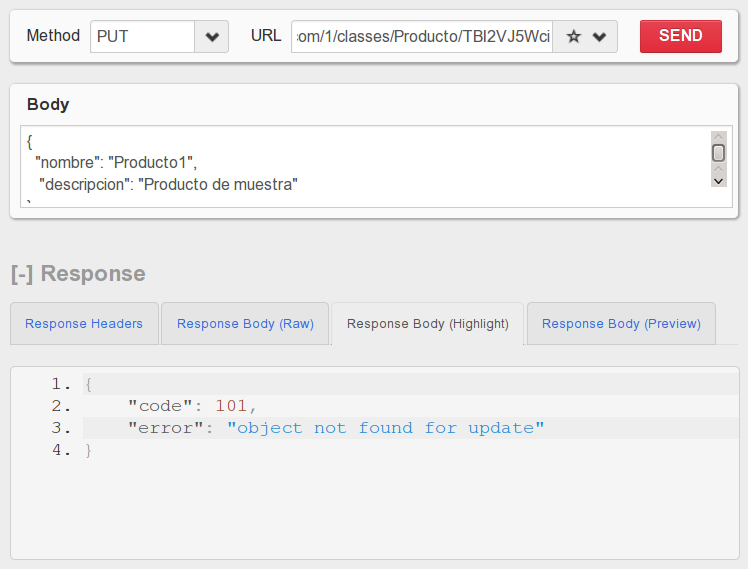
\includegraphics[width=0.9\textwidth]{imagenes/implementacion/acl.png}
     \caption{Solicitud de modificación rechazada a un objeto existente utilizando REST Client}
    \label{fig:acl}
\end{figure}

Esta medida de seguridad debe ser controlada en el servidor web que recibe las peticiones, debido a que controlarlo en el cliente no soluciona el problema de las modificaciones no autorizadas. Una solicitud a un objeto sin usar las credenciales de un usuario autorizado debe ser denegada por el servidor, como se muestra en la figura \ref{fig:acl}. Es importante también que el mensaje retornado por el servidor, en caso de que el objeto no tenga permisos de visualización por el usuario actual, no revele evidencia de la existencia del objeto.

\section{Backbone.js}

Backbone.js es un \gls{framework} para Javascript con un interfaz RESTful por \gls{JSON} , basada en el paradigma de diseño de aplicaciones Modelo Vista Presentador (MVP).
Está diseñado para desarrollar aplicaciones de una única página y para mantener las diferentes partes de las aplicaciones web (p.e. múltiples clientes y un servidor) sincronizadas.

Backbone.js posee cuatro clases principales:

\begin{itemize}
    \item Model 
    \item View
    \item Router
    \item Collection
 \end{itemize}
 
 \subsection{Modelo Vista Presentador (MVP)}
 
 El patrón Modelo-Vista-Presentador (MVP) surge como una variación del patrón Modelo-Vista-Controlador (MVC).
 
 Los componentes básicos de este patrón son:
 
\begin{figure}[htbp]
  \centering
    %lo que agregué entre corchetes hace que el ancho de la imagen ocupe el 80% del área de texto. Si sacás eso la imagen no se redimensiona y se va de la hoja. Se puede usar algo parecido para limitar el alto si es necesario.
    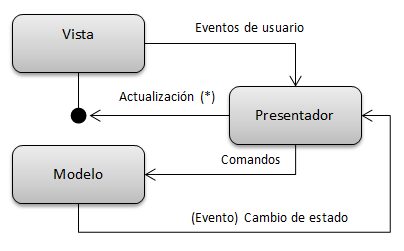
\includegraphics{imagenes/MVP.png}
    
     \caption{Componentes MVP}
    \label{MVP}
\end{figure}

 \begin{itemize}
    \item \emph {Modelo:} El modelo es normalmente los datos de la aplicación y la lógica para recuperar y conservar los datos. A menudo, se trata de un modelo de dominio que puede basarse en una base de datos o los resultados de los servicios web. En algunos casos, que el modelo de dominio corresponde perfectamente a lo que se ve en la pantalla, pero en otros casos ha de ser adaptada, agregados o extendido para ser utilizable.
    
    \item \emph {Vista:} La vista es típicamente un control de usuario o formulario que combina varios en una interfaz de usuario. El usuario puede interactuar con los controles en la vista
    %, pero cuando se necesita cierta lógica para iniciarse, la vista este delegado al presentador.
    
   \item \emph {Presentador:} El presentador tiene toda la lógica de la vista y es responsable de sincronizar el modelo y la vista. Cuando la vista notifica el presentador que el usuario ha hecho algo (por ejemplo, hacer clic en un botón), el presentador a continuación, actualizar el modelo y sincronizar los cambios entre el modelo y la vista.

      
 \end{itemize}


\section{jQuery}

jQuery es una biblioteca de \gls{JavaScript} que permite simplificar la manera de interactuar con los documentos \gls{HTML}, manipular el árbol \gls{DOM}, manejar eventos, desarrollar animaciones y agregar interacción con la técnica \gls{AJAX} a páginas web.

Es software libre y de código abierto, posee un doble licenciamiento bajo la Licencia MIT y la Licencia Pública General de GNU v2, permitiendo su uso en proyectos libres y cerrados.

Al igual que otras bibliotecas, ofrece una serie de funcionalidades basadas en JavaScript que de otra manera requerirían de mucho más código, es decir, con las funciones propias de esta biblioteca se logran grandes resultados en menos tiempo y líneas de código.

\section{jQuery Mobile}
jQuery Mobile es un \gls{framework} para Javascript utilizado en el desarrollo de la interfaz de usuario para aplicaciones web adaptadas a dispositivos móviles. Incluye elementos de UI y soporte a eventos relacionados con el uso de pantallas táctiles.

Las principales características de jQuery Mobile son:

\begin{itemize}
    \item Es compatible con otros frameworks que utilizamos para el desarrollo de la aplicación móvil, tales como Phonegap o Backbone.js.
    \item Es compatible con las principales plataformas móviles, así como todos los navegadores de escritorio principales, incluyendo Android.
    \item Construido sobre jQuery.
    \item Permite la creación de temas personalizados mediante el agregado de estilos CSS. Proporciona además una base de temas que permite a los desarrolladores personalizar las combinaciones de colores y determinados aspectos de las características de interfaz de usuario.
    \item Tiene mínimas dependencias, aumentando la velocidad y reduciendo el consumo de memoria.
    \item Adaptación automática del diseño al tamaño de la pantalla.
 \end{itemize}
 

\section{Herramientas de desarrollo}

\begin{itemize}

\item \emph {Eclipse:} Es un entorno de desarrollo integrado (IDE) de código abierto multiplataforma.

\item \emph {Visual Paradigm para UML:} Es una herramienta UML profesional que soporta el ciclo de vida completo del desarrollo de software: análisis y diseño orientados a objetos, construcción, pruebas y despliegue. 

Permite dibujar todos los tipos de diagramas de clases, código inverso, generar código desde diagramas y generar documentación.

\item \emph{\LaTeX:} Es un sistema de composición de textos, orientado especialmente a la creación de libros, documentos científicos y técnicos que contengan fórmulas matemáticas.

\LaTeX facilita el uso del lenguaje de composición tipográfica. Es muy utilizado para la composición de artículos académicos, tesis y libros técnicos, dado que la calidad tipográfica de los documentos realizados con \LaTeX es comparable a la de una editorial científica de primera línea.



\item \emph{ShareLaTeX:} Es un editor online (en tiempo real)de \LaTeX, que puede ser utilizado por varios usuarios a la vez. 

\item \emph{Dropbox y Google Drive:} Son servicios de alojamiento de archivos multiplataforma en la nube, operado por las compañías Dropbox y Google. 

Permiten a los usuarios almacenar y sincronizar archivos en línea y entre computadoras y compartir archivos y carpetas con otros.

\end{itemize}

